\onehalfspacing
\begin{refsection}
\chapter[Introduction]{Introduction}
\label{ch:introduction}

Aliquam erat volutpat. Nam iaculis euismod urna. Ut neque lacus, condimentum dignissim sem ac, elementum lacinia quam. Vestibulum a dictum justo, non dignissim ipsum. Donec massa nunc, suscipit in tincidunt a, efficitur ac eros. Nulla nec eros elementum, feugiat velit vitae, hendrerit lacus. Curabitur tortor leo, cursus vel ante hendrerit, vulputate fermentum nisl. Praesent fringilla vitae ante at molestie. Nullam lacinia nibh eget rhoncus tristique.

A citation, either \citep{Massonet1998} or \citet{Massonet1998}

\begin{equation}
	Binary \ output =
  \begin{cases}
    1 & \text{if $\textbf{w}.\textbf{x}  > threshold$}\\
    0 & \text{if $\textbf{w}.\textbf{x} \leq threshold$}\\
  \end{cases}
\end{equation}


\section{A section}
\label{sec:volcano_monitoring_and_insar}


\begin{figure}[tbp]
	\centering
	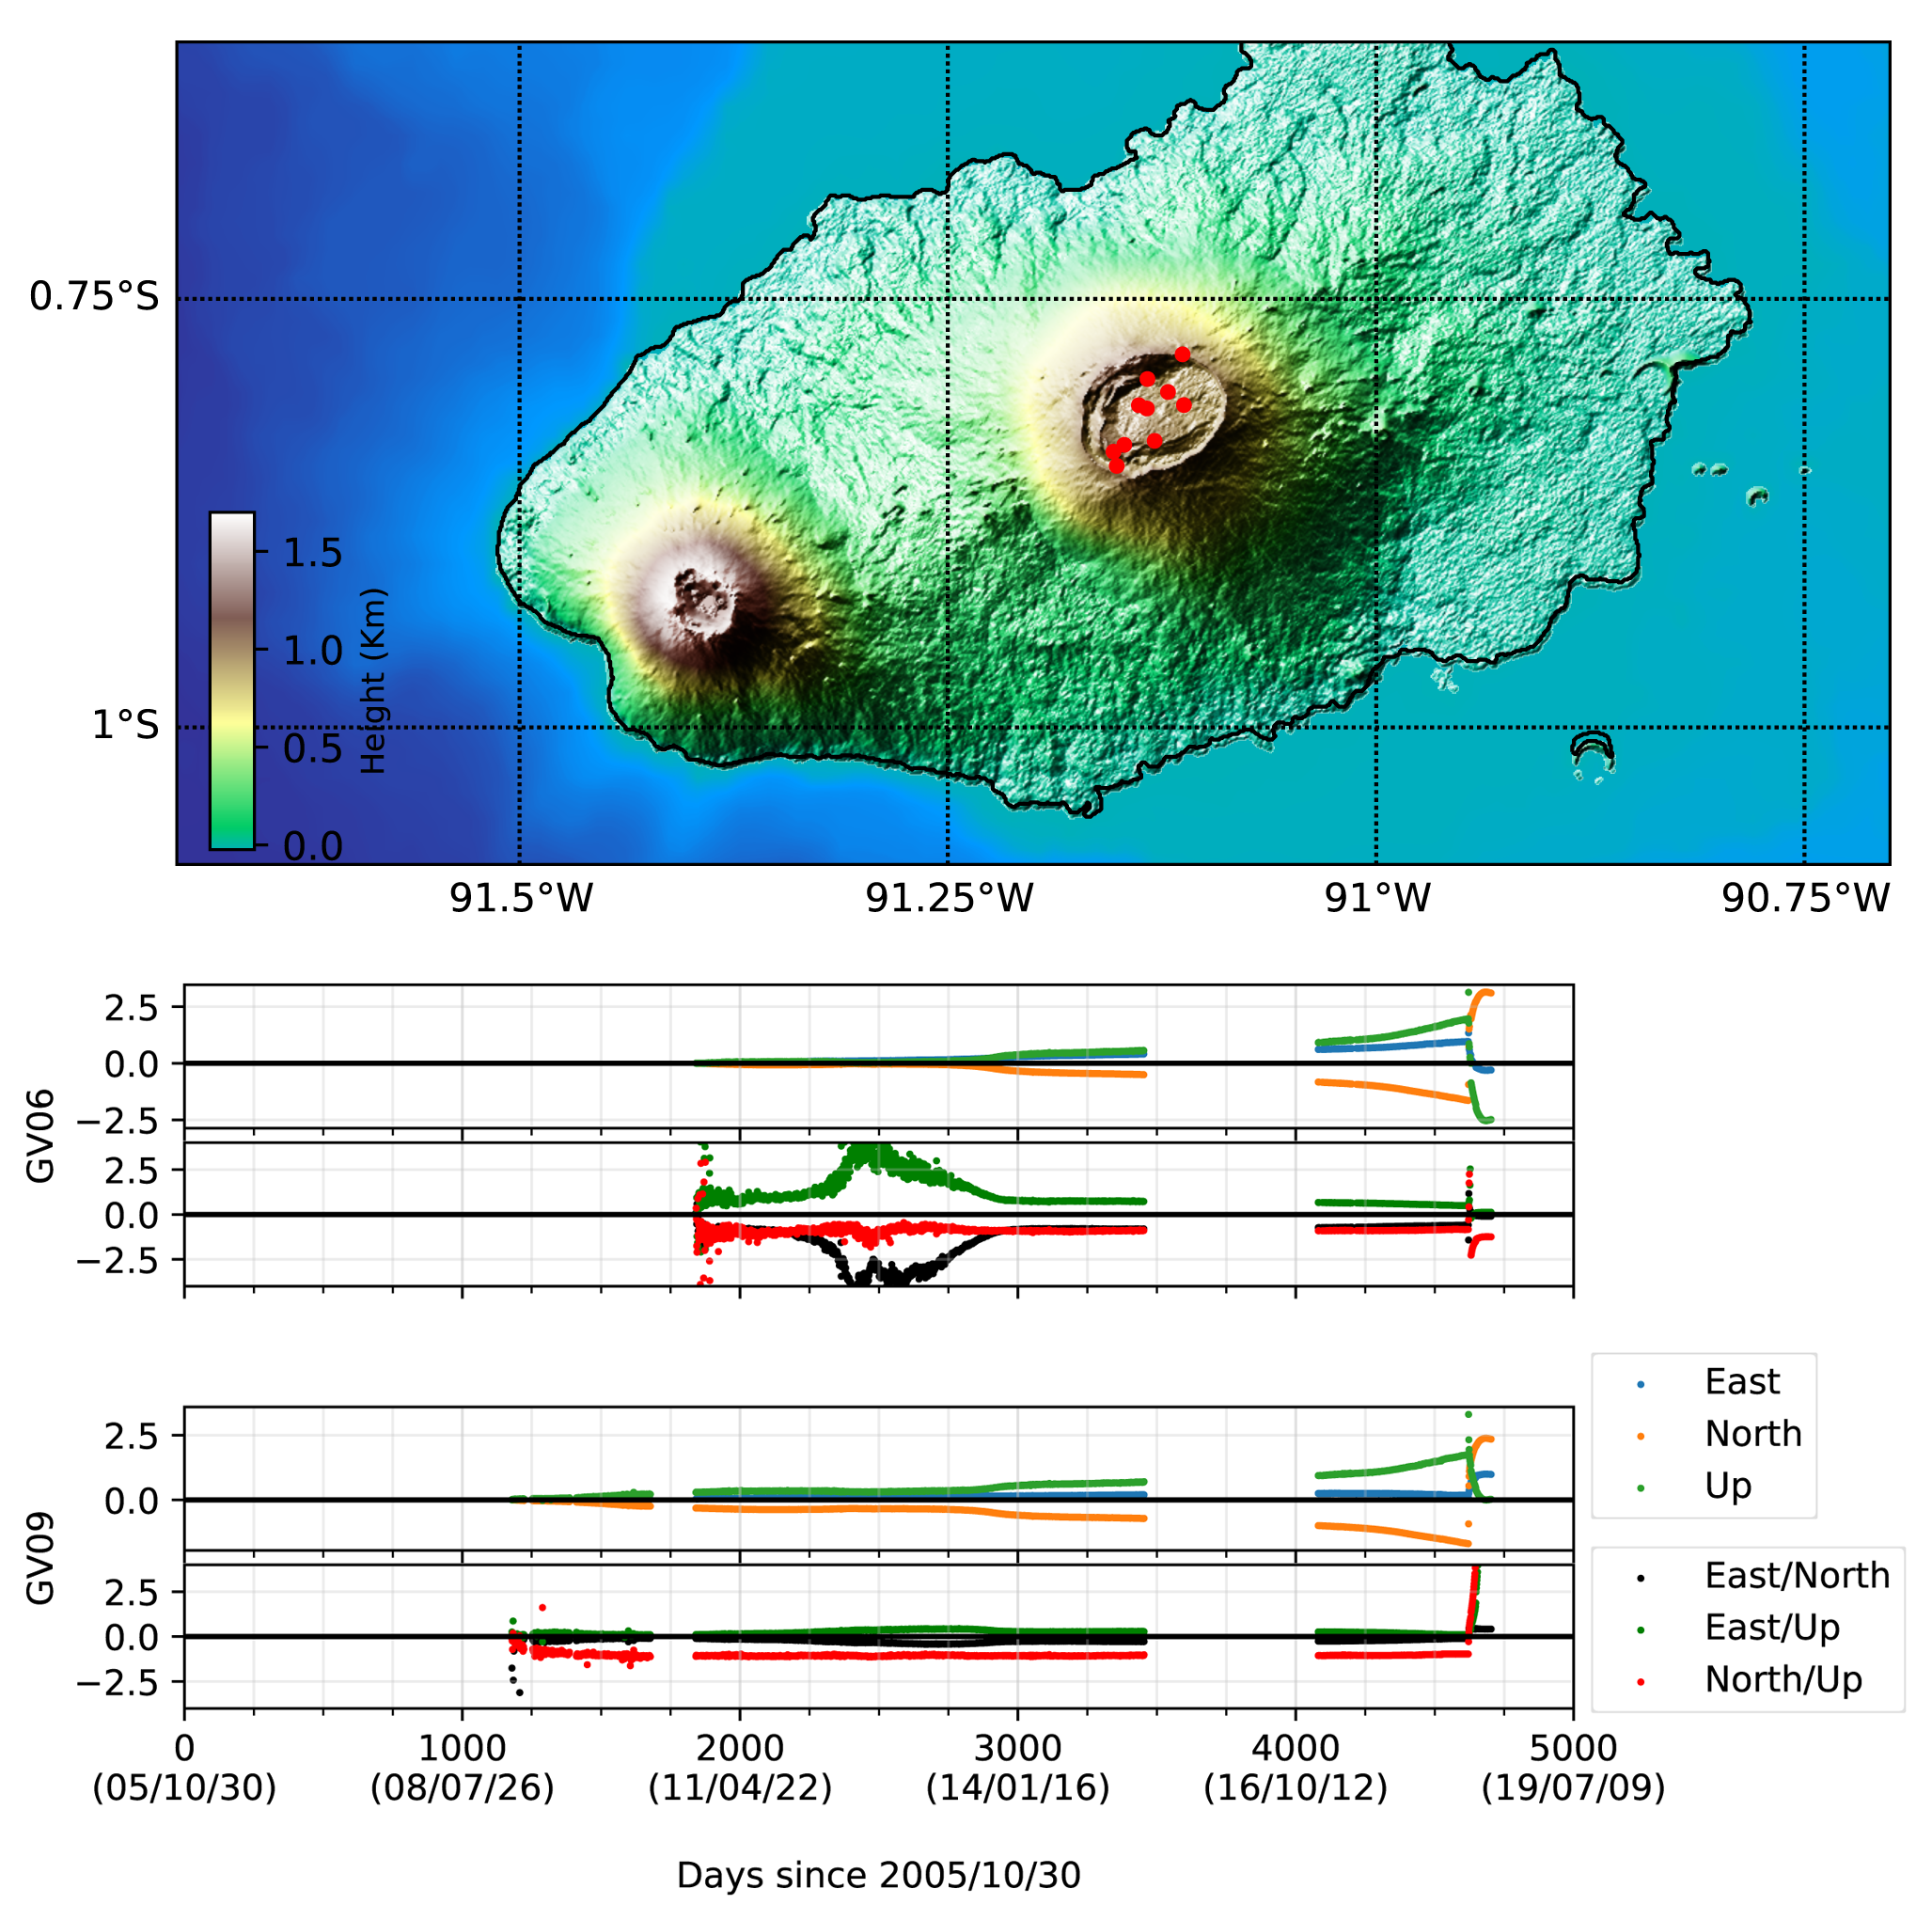
\includegraphics[width=1\textwidth]{./front_material_figures/figure_3_sn_gps.png}
	\caption[Short Caption]{Long caption}
	\label{fig:population_volcanoes}
\end{figure}





\section{Aims and Objectives}
\label{sec:aims}
Mauris venenatis vitae tellus pharetra luctus. Donec egestas, neque at faucibus tincidunt, lorem ex accumsan nibh, sed lobortis magna leo ac lorem. Fusce luctus nibh et eros malesuada volutpat. Donec gravida ultrices ornare. Fusce maximus magna tortor, at tristique lectus mollis nec. Proin hendrerit rutrum tortor, eget varius velit ornare ut. Vestibulum hendrerit neque non venenatis tristique. Cras id ullamcorper tortor.

The objectives of this thesis are:

\begin{enumerate}
	\item{Objective 1}
	\item{Objective 2}
	\item{Objective }
\end{enumerate}




\section{Thesis outline}
\label{sec:outline}
The subsequent chapters in this thesis are organised as follows:

\begin{itemize}
  \item Chapter \ref{ch:publication1} blah blah.

  \item Chapter \ref{ch:publication2} more blah.

  \item Chapter \ref{ch:publication3} blah 3.


  \item Chapter \ref{ch:back_material} discusses the work contained within the preceding chapters in relation to the goal of Blah.
\end{itemize}



\printbibliography[heading=subbibliography]
\end{refsection}
\cleardoublepage
